\documentclass[border=10pt]{standalone}
\usepackage{amsmath}
\usepackage{amssymb}
\usepackage{tikz}
\usetikzlibrary{arrows.meta,calc,decorations.pathreplacing,patterns,shapes.geometric,positioning,shadings,plotmarks}

\begin{document}
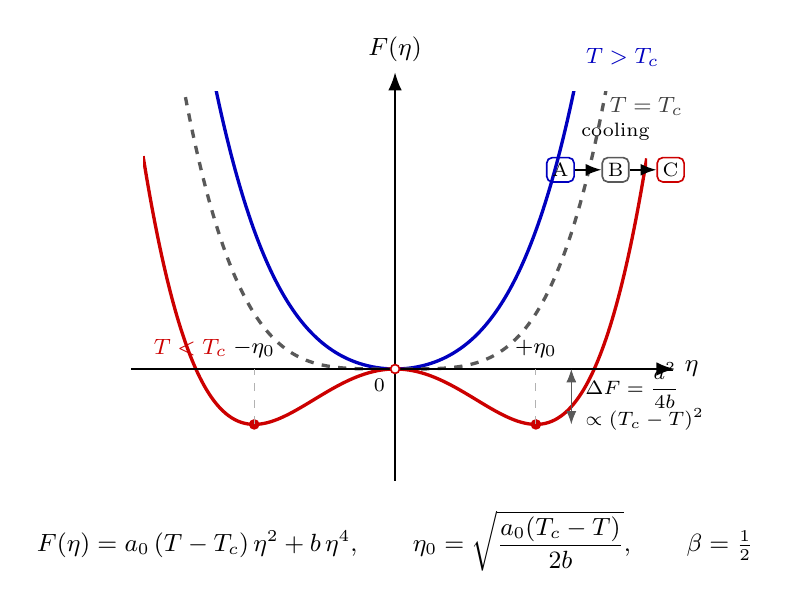
\begin{tikzpicture}[>=Latex, line width=0.6pt, font=\small,
  declare function={
    % Curve A: T > Tc, a = +0.6, b = 0.5: F = 0.6*x^2 + 0.5*x^4
    fA(\x) = 0.6*\x*\x + 0.5*\x*\x*\x*\x;
    % Curve B: T = Tc, a = 0, b = 0.5: F = 0.5*x^4
    fB(\x) = 0.5*\x*\x*\x*\x;
    % Curve C: T < Tc, a = -0.8, b = 0.5: F = -0.8*x^2 + 0.5*x^4
    fC(\x) = -0.8*\x*\x + 0.5*\x*\x*\x*\x;
  }
]

% --- Coordinate system ---
% x-range roughly [-1.6, 1.6], y-range scaled by 1.4
\def\xmin{-1.6}
\def\xmax{1.6}
\def\xscale{2.0}    % horizontal scale: 2 cm per eta unit
\def\yscale{2.2}    % vertical scale: 2.2 cm per F unit
\def\ymin{-0.6}
\def\ymax{1.6}

% Helper: clip box for the curves
\begin{scope}
  \clip ({\xscale*(\xmin)},{\yscale*(\ymin)}) rectangle ({\xscale*(\xmax)},{\yscale*(\ymax)});

  % --- Curve A: single well, blue (T > Tc) ---
  \draw[blue!75!black, very thick, domain=\xmin:\xmax, samples=120, smooth, variable=\x]
    plot ({\xscale*\x},{\yscale*fA(\x)});

  % --- Curve B: flat-bottom quartic, gray (T = Tc) ---
  \draw[gray!70!black, very thick, dashed, domain=\xmin:\xmax, samples=120, smooth, variable=\x]
    plot ({\xscale*\x},{\yscale*fB(\x)});

  % --- Curve C: double well, red (T < Tc) ---
  \draw[red!80!black, very thick, domain=\xmin:\xmax, samples=160, smooth, variable=\x]
    plot ({\xscale*\x},{\yscale*fC(\x)});
\end{scope}

% --- Axes (drawn after curves so labels stay clear) ---
% Horizontal axis (eta)
\draw[->, line width=0.8pt] ({\xscale*(\xmin)-0.15},0) -- ({\xscale*(\xmax)+0.35},0)
  node[right] {$\eta$};
% Vertical axis (F)
\draw[->, line width=0.8pt] (0,{\yscale*(\ymin)-0.1}) -- (0,{\yscale*(\ymax)+0.25})
  node[above] {$F(\eta)$};

% Origin label
\node[below left, font=\scriptsize] at (0,0) {$0$};

% --- Mark the two minima of curve C (eta_0 = sqrt(0.8)) ---
% eta_0 = sqrt(0.8) approx 0.8944; F_min = -0.8*0.8 + 0.5*0.64 = -0.64 + 0.32 = -0.32
\def\etazero{0.8944}
\def\Fmin{-0.32}

\filldraw[red!80!black] ({\xscale*(\etazero)},{\yscale*(\Fmin)}) circle (1.6pt);
\filldraw[red!80!black] ({-\xscale*(\etazero)},{\yscale*(\Fmin)}) circle (1.6pt);

% Origin (local maximum on curve C) marker
\filldraw[red!80!black, fill=white, line width=0.6pt]
  (0,0) circle (1.6pt);

% Labels for +/- eta_0 on x-axis
\draw[dashed, gray!60, line width=0.4pt]
  ({\xscale*(\etazero)},{\yscale*(\Fmin)}) -- ({\xscale*(\etazero)},0);
\draw[dashed, gray!60, line width=0.4pt]
  ({-\xscale*(\etazero)},{\yscale*(\Fmin)}) -- ({-\xscale*(\etazero)},0);

\node[above, font=\footnotesize] at ({\xscale*(\etazero)},0.02) {$+\eta_0$};
\node[above, font=\footnotesize] at ({-\xscale*(\etazero)},0.02) {$-\eta_0$};

% --- Annotation: bump height Delta F = a^2/(4b) ---
% On curve C, depth from origin to F_min: |F_min| = 0.32
\draw[<->, line width=0.4pt, gray!70!black]
  ({\xscale*(\etazero)+0.45},0) -- ({\xscale*(\etazero)+0.45},{\yscale*(\Fmin)});
\node[right, font=\scriptsize, align=left] at ({\xscale*(\etazero)+0.5},{0.5*\yscale*(\Fmin)})
  {$\Delta F=\dfrac{a^2}{4b}$\\[-1pt]\scriptsize $\propto(T_c-T)^2$};

% --- Curve labels ---
% Curve A label (top right of blue curve)
\node[blue!75!black, font=\footnotesize, anchor=south west]
  at ({\xscale*1.15},{\yscale*fA(1.15)+0.05}) {$T>T_c$};

% Curve B label (along quartic, mid range)
\node[gray!50!black, font=\footnotesize, anchor=south west]
  at ({\xscale*1.30},{\yscale*fB(1.30)-0.05}) {$T=T_c$};

% Curve C label (in the well region, below origin)
\node[red!80!black, font=\footnotesize] at ({-\xscale*1.30},{\yscale*fC(1.30)+0.10}) {$T<T_c$};

% --- Bottom: model formula and beta ---
\node[anchor=north, font=\small] at (0,{\yscale*(\ymin)-0.35})
  {$F(\eta)=a_0\,(T-T_c)\,\eta^2+b\,\eta^4,\qquad
    \eta_0=\sqrt{\dfrac{a_0(T_c-T)}{2b}},\qquad \beta=\tfrac12$};

% --- Cooling-arrow chain A -> B -> C in upper right ---
\begin{scope}[shift={({\xscale*1.05},{\yscale*1.15})}, font=\scriptsize]
  \node[draw=blue!75!black, rounded corners=2pt, inner sep=2pt] (LA) at (0,0) {A};
  \node[draw=gray!70!black, rounded corners=2pt, inner sep=2pt] (LB) at (0.7,0) {B};
  \node[draw=red!80!black, rounded corners=2pt, inner sep=2pt] (LC) at (1.4,0) {C};
  \draw[->, >=Latex] (LA) -- (LB);
  \draw[->, >=Latex] (LB) -- (LC);
  \node[anchor=south, font=\scriptsize] at (0.7,0.25) {cooling};
\end{scope}

\end{tikzpicture}
\end{document}
